\documentclass[a4paper,12pt]{letter} 

\usepackage{amsmath}
\usepackage{amssymb}
\usepackage{nopageno}
\usepackage{amsmath}
%\usepackage{enumitem}
% \usepackage{mathtools}
%\usepackage{eqnarray,amsmath}
\usepackage[a4paper, total={7.5in, 11.25in}]{geometry}
%\usepackage[margin=2.5cm]{geometry}
\usepackage[utf8]{inputenc}
\usepackage[T1]{fontenc}
\usepackage{lmodern}
%\usepackage{amsmath, amssymb}
\usepackage{setspace}
\setstretch{1.2}
\usepackage{pgfplots}
\pgfplotsset{compat=1.18}

\begin{document}

\begin{center}
\textbf{\huge Analysis of Hungarian Pensions}
\end{center}

\vspace{10pt}

Data of the given frequency distribution ($x_i$: pension amount, $f_i$: number of pensioners):

\begin{center}
\begin{tabular}{|c|cccccc|}
\hline
$x_i$ [kHUF] & 50 & 150 & 250 & 350 & 450 & 550 \\ \hline
$f_i$ & 200 & 1000 & 675 & 270 & 100 & 60 \\ \hline
\end{tabular}
\end{center}

Total sample size ($N$): $$ N = \sum f_i = 200 + 1000 + 675 + 270 + 100 + 60 = \mathbf{2305}$$

The expected value is the weighted arithmetic mean: $$\mu = \frac{\sum (x_i \cdot f_i)}{N}= \frac{(50 \cdot 200) + (150 \cdot 1000) + (250 \cdot 675) + (350 \cdot 270) + (450 \cdot 100) + (550 \cdot 60)}{2305} =$$ $$ =\frac{501,250}{2305} \approx \mathbf{217.46}$$

The standard deviation is the square root of the average squared deviations: $$\sigma = \sqrt{\frac{\sum f_i \cdot (x_i - \mu)^2}{N}} = \sqrt{\frac{200(50-217.46)^2 + 1000(150-217.46)^2 + \dots + 60(550-217.46)^2}{2305}} \approx$$ $$ \approx \sqrt{11,564.37} \approx \mathbf{107.54}$$

\begin{center}
  \bigskip
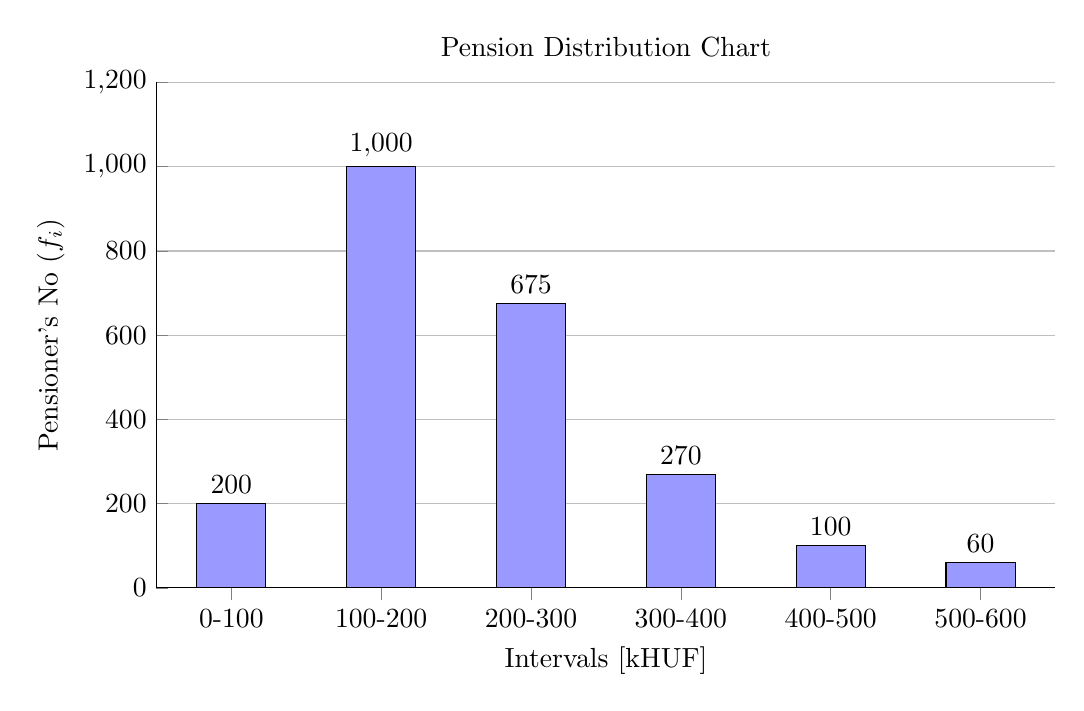
\begin{tikzpicture}
\begin{axis}[
    ybar,
    bar width=25pt,
    title={Pension Distribution Chart},
    xlabel={Intervals [kHUF]},
    ylabel={Pensioner's No ($f_i$)},
    symbolic x coords={0-100, 100-200, 200-300, 300-400, 400-500, 500-600},
    xtick=data,
    nodes near coords,
    ymin=0,
    ymax=1200,
    width=13cm,
    height=8cm,
    axis lines*=left,
    ymajorgrids=true,
]
\addplot[fill=blue!40] coordinates {
    (0-100,200) (100-200,1000) (200-300,675) (300-400,270) (400-500,100) (500-600,60)
};
\end{axis}
\end{tikzpicture}
\end{center}

\end{document}
